
\chapter{Oscillation libre dans un circuit RLC}
\section{Décharge oscillante d'un condensateur dans une bobine idéale}
\subsection{Expression de la tension}

\begin{figure}[!htb]
    \centering
    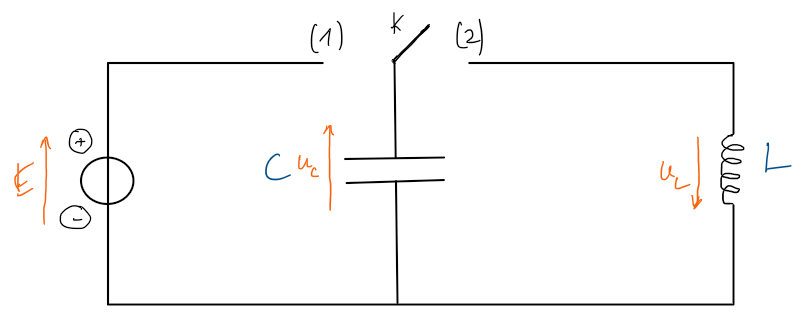
\includegraphics[width=0.5\textwidth]{SCHEMA1.png}
    \caption{Schema de montage}
    \label{fig:SCHEMA1}
\end{figure}


A \(t = O\)s, on a \(u_{c}(0) = E\) et \(i(0) = 0\)A et on bascule \(K\) en position 2. 

\begin{figure}[!htb]
    \centering
    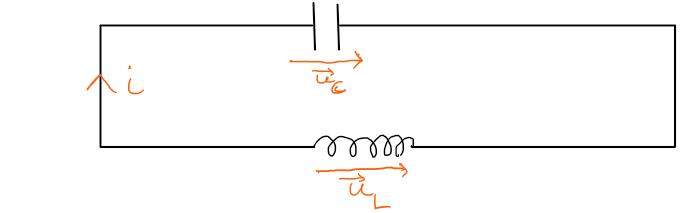
\includegraphics[width=0.5\textwidth]{SCHEMA2.png}
    \caption{Schema du montage à \(t=0 \unit{s}\)}
    \label{fig:SCHEMA2}
\end{figure}



D'après la loi des mailles :
\begin{eqnarray*}
    &&u_{L} + u_{C} = 0\\
    &&\iff L \frac{di}{dt} + u_{C} = 0\\
    &&\text{or } i = C \frac{du_{C}}{dt} \\
    &&\iff LC \frac{d}{dt}\left[ \frac{d}{dt}u_{c} \right] + u_{c} = 0\\
    &&\textnormal{On pose \(\omega_{0}^{2} = \frac{1}{LC}\) }\\
    &&\implies \frac{d^{2}u_{c}}{dt^{2}} + \omega_{0}^{2} u_{c} = 0
\end{eqnarray*}
On cheche l'unité de \(\left[ RC \right] = ?\)\\
\[
    \begin{cases}
        u_{l} = L \frac{di}{dt} \implies [L] = V \cdot s \cdot A^{-1}\\
        i = C \frac{du_{c}}{dt} \implies \left[ C \right] = A \cdot  s \cdot  V^{-1}
    \end{cases}
    \implies \left[ LC \right] = s^{2} \implies \left[ \omega_{0} \right] = s^{-1}
\] 

\begin{theorem}[Résolution d'équations différentielles du second ordre]\label{thm:ED2SSM}
        On considère une ED du second ordre, SSM, à coeficients constants : 
        \[
            ay'' + by' + cy = 0 \, , a \neq 0
        \]
        A cette ED, on associe le polynome caractéristique : \\
        \[
            ar^{2}+br+c = 0 \implies \Delta = b^{2}-4ac
        \]
        3 cas :\\
        \begin{itemize}
            \item Cas 1 : \(\Delta >0\)\\
                \(\exists, r_{1}, r_{2} \in \mathbb{R}\) solutions de léquations.\\
                \[
                    \begin{cases}
                        r_{1} = \frac{-b + \sqrt{\Delta}}{2a}\\
                        r_{2} = \frac{-b-\sqrt{\Delta}}{2a}
                    \end{cases}
                \]
                La solution de l'ED est : \(y = A e^{r_{1}x} + B e^{r_{2}x}\), avec \(A\) et \(B\) à déterminer. 
            \item Cas 2 : \(\Delta = 0\)\\
                \(\exists! r\) solution : \(r= -\frac{b}{2a}\).\\
                La solution de l'ED est : \(y = \left( A'x+B' \right)e^{rx}\) avec \(A'\) et \(B'\) à déterminer.
            \item Cas 3 : \(\Delta <0\) \\
                \(\exists r_{3}, r_{4} \in \mathbb{C}\) : \\
                \[
                    \begin{cases}
                        r_{3} = \frac{-b-j\sqrt{-\Delta }}{2a}\\
                        r_{4} = \frac{-b+j\sqrt{-\Delta}}{2a}
                    \end{cases} \text{ avec } j^{2} = -1
                \] 
                On a alors : 
                \begin{eqnarray*}
                    y &=& A'' e^{r_{3}x}+ B''e^{r_{4}x}\\
                    &=& \left( A'' \exp \left[ \frac{-j-\sqrt{-\Delta}}{2a} \right] + B''e^{\frac{-j+\sqrt{-\Delta }}{2a}} \right)e^{-\frac{b}{2a}x}\\
                    &=& \left( \alpha \cos (\frac{\sqrt{-\Delta}}{2a}x) + \beta \sin (\frac{\sqrt{-\Delta }}{2a}x ) \right)e^{-\frac{b}{2a}x}
                \end{eqnarray*}
        \end{itemize} 
\end{theorem}

On a : 
\[
    \frac{d^{2}u_{C}}{dt^{2}} + \omega_{0}^{2}u_{C} = 0
\]
L'équation charactéristique est donc :\\
\begin{eqnarray*}
    \implies r^{2} + \omega_{0}^{2} &=& 0 \\
    \implies \Delta &=& -4\omega_{0}^{2}\\
    \implies r &=& \pm j \frac{\sqrt{4\omega_{0}^{2}}}{2} = \pm j \omega_{0}\\
    \implies  u_{c}(t) &=& A \cos (\omega_{0} t) + B \sin (\omega_{0} t)\\ 
    \implies u_{c}(t) &=& A\cos \omega_{0}t + B \sin \omega_{0}t
\end{eqnarray*}

Pour trouver \(A\) et \(B\), on utilise les conditions initiales :\\
\[
    \begin{cases}
        u_{c}(0) = E\\
        i(0) = C\frac{d}{dt}(u_{c})(0) = 0
    \end{cases}
\]
\begin{eqnarray*}
    i(t) &=& C \left[ -A \omega_{0} \sin \omega_{0}t + B \omega_{0} \cos \omega_{0}t  \right]\\
    i(0) &=& 0 = CB \omega _{0} \implies B = 0 \\
    &&\text{De plus, } u_{c}(0) = E = A\\
    &\implies& u_{C}(t) = E\cos(\omega_{0}t)
\end{eqnarray*}

On sait que la période propre de l'oscillation \(T_{0}\) est celle t.q. : \\
\begin{eqnarray*}
    &&u_c(t+T_{0}) = u_{c}(t)\\
    &\implies& \cos (\omega_{0}(t+T_{0})) = \cos(t)\\
    &\implies& \cos(\omega_{0}t + \omega_{0}T_{0}) = \cos(t)\\
    &&\text{Or cos est } 2\pi \text{ périodique}\\
    &\implies& \omega _{0} T_{0} = 2\pi \implies \omega _{0} = \frac{2\pi}{T_{0}} = 2\pi f_{0}\\
    &&\text{Or, } \omega_{0} = \frac{1}{\sqrt{LC}} = \frac{2\pi}{T_{0}}\\
    &\implies& T_{0} = 2\pi\sqrt{LC}, \text{ On appelle } T_{0} \text{ la période propre de l'oscillateur.}
\end{eqnarray*}

\begin{figure}[!htb]
    \centering
    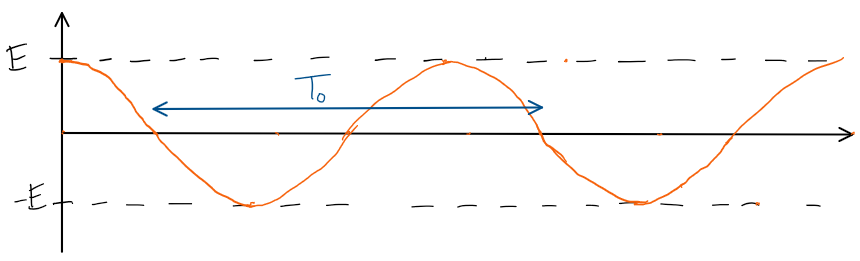
\includegraphics[width=1\textwidth]{SCHEMA3.png}
    \caption{Schema de \(u_{c} (\text{ en } \unit{V})\) en fonction du temps }
    \label{fig:SCHEMA3}
\end{figure}


Et pour \(i(t)\)?\\
\begin{eqnarray*}
    i(t) &=& C \frac{d}{dt}u_{c}(t) = C \frac{d}{dt}E\cos (\omega _{0}t)\\
    i(t) &=& -\omega_{0}CE\sin \omega_{0}t\\
     &=& -\frac{CE}{\sqrt{LC}} \sin(\omega _{0}t) \\
     i(t) &=& -\sqrt{\frac{C}{L}}E\sin (\omega_{0}t)\\
     i(t) &=& -\sqrt{\frac{C}{L}}E\cos(2\pi-\omega_{0}t) 
\end{eqnarray*}

\begin{figure}[!htb]
    \centering
    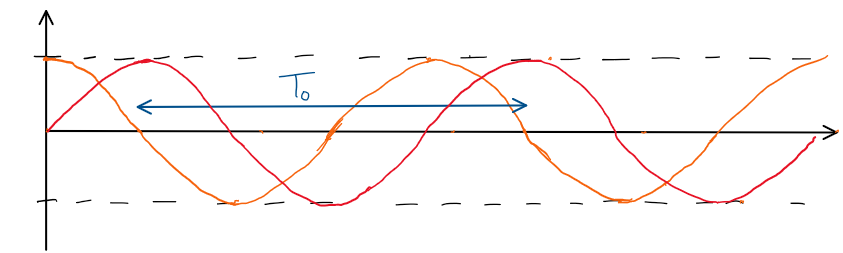
\includegraphics[width=1\textwidth]{SCHEMA4.png}
    \caption{Représentation de \(u_{c}\) et \(i\) en fonction du temps }
    \label{fig:SCHEMA4}
\end{figure}


Lorque \(u_{c}(t) = 0\), \(i(t)\) est maximale ou minimale. On dit que \(u_{c}(t)\) et \(i(t)\) sont en quadrature de phase. 

\subsection{Approche énergétique}

Pour tout instant \(t\), \(E_{tot}\) est la somme des énergies enmagasinées par la bobine et le condensateur.\\
\begin{eqnarray*}
    E_{em} &=& E_{c} + E_{m}\\
    &=& \frac{1}{2}cu_{c}^{2} + \frac{1}{2}Li^{2}\\
    &&\text{Or }i(t) = C\frac{d}{dt}u_{c}(t)\\
    \frac{d}{dt}E_{em} &=& \frac{d}{dt}\left[ \frac{1}{2}Cu_{c}^{2} + \frac{1}{2}Li^{2} \right]\\
    &=& \frac{1}{2} C 2u_{c}\frac{d}{dt}u_{c} + \frac{1}{2}L 2 i \frac{d}{dt}i\\
    &=& \left[ u_{c} + LC \frac{d^{2}u_{c}}{dt^{2}} \right] \cdot i\\
    &=& 0 \,(\text{car le membre de gauche dans le produit est nul})\\
    & \implies& E_{em} = \frac{1}{2}Li^{2} + \frac{1}{2}Cu_{c}^{2} = \text{ cste}
\end{eqnarray*}

\begin{remark}[Parallèle avec la mécanique]
    On peut faire un parallèle avec les oscillateurs harmoniques en mécanique (par exemple, la masse au bout du ressort) : \\
    \[
        E_{m} = \frac{1}{2}m \dot{x} + \frac{1}{2}kx^{2}
    \]
\end{remark}

\begin{figure}[!htb]
    \centering
    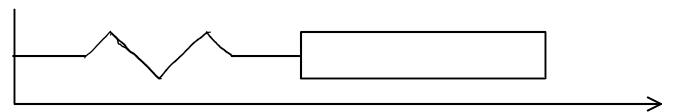
\includegraphics[width=0.5\textwidth]{SCHEMA5.png}
    \caption{Analogie avec le ressort}
    \label{fig:SCHEMA5}
\end{figure}


\section{Décharge dans un résistor}

\begin{figure}[!htb]
    \centering
    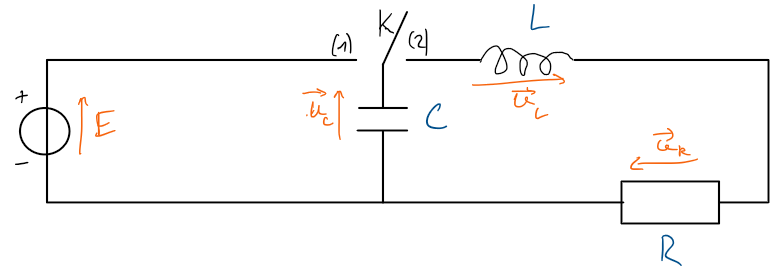
\includegraphics[width=0.5\textwidth]{SCHEMA6.png}
    \caption{Schema du montage}
    \label{fig:SCHEMA6}
\end{figure}


A \(t  =0\)s, on bascule l'interrupteur en position 2. On a : 
\begin{eqnarray*}
    u_{c}(0) &=& E \\
    i(0) &=& 0
\end{eqnarray*}

\begin{figure}[!htb]
    \centering
    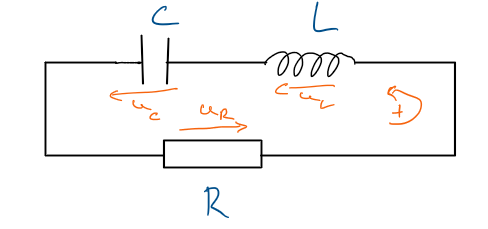
\includegraphics[width=0.5\textwidth]{SCHEMA7.png}
    \caption{Schema du montage à \(t = 0 \unit{s}\) }
    \label{fig:SCHEMA7}
\end{figure}


D'après la loi des mailles : 
\begin{eqnarray*}
    u_{L} + u_{R} + u_{C} &=& 0 \\
    \iff u_{C} + ri + L \frac{di}{dt} &=& 0 \\
    \text{ Or :  } u_{C} = \frac{q}{C} \text{ et } i &=& \frac{dq}{dt} \implies  i = C \frac{du_{c}}{dt} \\
    \iff LC \frac{d^{2}u_{c}}{dt^{2}} + RC \frac{du_{c}}{dt} + u_{c} &=& 0
\end{eqnarray*}

\begin{notation}
    A partir de maintenant on notera : 
    \[
        u = u_{c} \implies \dot{u} = \frac{du_{c}}{dt} \wedge \ddot{u} = \frac{d^{2}u_{c}}{dt^{2}}
    \]
\end{notation}

On a : 
\[
    \ddot{u} + \frac{R}{L}\dot{u} + \frac{1}{LC}u = 0
\]

\begin{notation}
    On pose : \(\omega_{\text{0}}^{2} = \frac{1}{LC}\) et \(2\lambda  = \frac{R}{L}\).   
\end{notation}
D'où : 
\[
    \ddot{u} + 2\lambda \dot{u} + \omega_{\text{0}}^{2} u = 0
\]
On associe l'équation caractéristique : 

\begin{eqnarray*}
    r^{2} + 2\lambda r + \omega_{\text{0}}^{2} &=& 0 \\
    \implies \Delta &=& 4\lambda^{2} -4\omega_{\text{0}}^{2} = 4(\lambda^{2} - \omega_{\text{0}}^{2}) \\
\end{eqnarray*}

\begin{remark}[Régime critique]
    Si \(\Delta = 0\) alors, on a le régime critique : \(\lambda = \omega_{\text{0}}\). \par
    Alors : \(\frac{R}{2L} = \frac{1}{\sqrt{LC}} \implies R = 2\sqrt{\frac{L}{C}}\). C'est la valeur de la résistance pour laquelle la décharge et la plus rapide.   

\end{remark}

On traite alors le cas où : \(\Delta <0\). \par
\begin{eqnarray*}
    r &=& \frac{-2\lambda \pm 2 j \sqrt{\omega_{\text{0}}^{2}-\lambda^{2}}}{2} \\
    r &=& -\lambda \pm j\sqrt{\omega_{\text{0}}^{2}-\lambda^{2}}
\end{eqnarray*}

On a un régime pseudo périodique : 
\[
    u(t) = A \cos (\sqrt{\omega_{\text{0}}^{2}-\lambda^{2}}t)e^{ -\lambda t } + B \sin ( \sqrt{\omega_{\text{0}}^{2}-\lambda^{2}} t ) e^{ -\lambda t }
\]
On trouve des valeurs des constantes inconnues en utilisant les conditions initiales : 
\begin{eqnarray*}
    u(0) &=& E \implies A = E \\
    i(t) &=& \frac{du}{dt} \\
    &=& \frac{d}{dt}\left[e^{ -\lambda t }\left(E\cos (\sqrt{\omega_{\text{0}}^{2}-\lambda^{2}} t) B\sin(\sqrt{\omega_{\text{0}}^{2}-\lambda^{2}})\right)\right] \\
    &=& -\lambda e^{ \lambda t } \left(  E\cos (\sqrt{\omega_{\text{0}}^{2}-\lambda^{2}} t) B\sin(\sqrt{\omega_{\text{0}}^{2}-\lambda^{2}})\right)  \\
    && + \, \, \, e^{ -\lambda t } \left( -E\sqrt{\omega_{\text{0}}^{2}-\lambda^{2}} \sin \left( \sqrt{\omega_{\text{0}}^{2}-\lambda^{2}} \right) + B \sqrt{\omega_{\text{0}}^{2}-\lambda^{2}} \cos \left( \sqrt{\omega_{\text{0}}^{2}-\lambda^{2}} \right)\right)\\
    \text{ Or :  } i(0) &=& 0 \\
    \implies B\sqrt{\omega_{\text{0}}^{2}-\lambda^{2}} - \lambda E &=& 0 \\
    \implies  B &=& \frac{\lambda E}{\sqrt{\omega_{\text{0}}^{2}-\lambda^{2}}}
\end{eqnarray*}

On peut définir une pseudo période propre : 
\[
    T_{0}  =\frac{2\pi}{\sqrt{\omega_{\text{0}}^{2}-\lambda^{2}}}
\]

\begin{figure}[!htb]
    \centering
    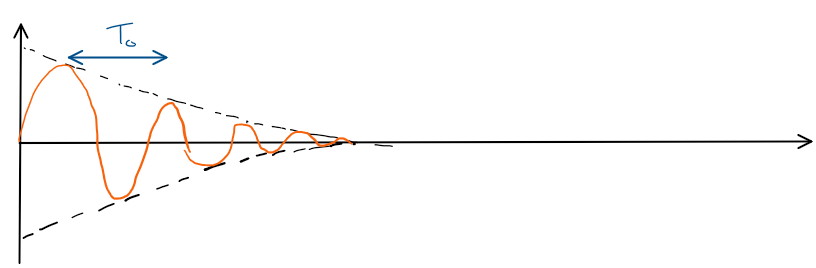
\includegraphics[width=0.8\textwidth]{SCHEMA8.png}
    \caption{Représentation de \(u_{c}\) en fonction du temps }
    \label{fig:SCHEMA8}
\end{figure}


D'ou on a : 
\[
    u(t) = \left[ E \cos \left( \sqrt{\omega_{\text{0}}^{2}-\lambda^{2} t} \right) + \frac{\lambda E}{\sqrt{\omega_{\text{0}}^{2}-\lambda^{2}}} \sin \left( \sqrt{\omega_{\text{0}}^{2}-\lambda^{2}} t \right) \right]
\]

\subsubsection{Aspect énergétique}

\begin{definition}[L'énergie mécanique en électromagnétique]
    On définit ainsi l'énergie électro magnétique du système : 
    \begin{eqnarray*}
        E_{em} &=& E_{e} + E_{m} \\
        &=& \frac{1}{2}Cu^{2} + \frac{1}{2}Li^{2}
    \end{eqnarray*}
\end{definition}

\begin{corollary}[Variation de l'énergie électromagnétique]
    Dans le cas de la décharge dans un résistor, on a : 
    \[
        \frac{dE_{em}}{dt} = -Ri^{2}
    \]
    Donc l'énergie du système tends vers \(0\).
\end{corollary}

\begin{explanation}
    \begin{eqnarray*}
        E_{em} &=& \frac{1}{2}Cu^{2} + \frac{1}{2}Li^{2} \\
        \implies \dot{E}_{em} &=& \frac{dE_{em}}{dt} \\
        &=& \frac{d}{dt}\left[ \frac{1}{2}Cu^{2} \right] + \frac{d}{dt}\left[ \frac{1}{2}Li^{2} \right] \\
        &=& \frac{1}{2}Cu\dot{u} 2 + \frac{1}{2}L 2 i \dot{i}\\
        &=& i \left[ L \frac{di}{dt} + u \right] \\
        &=& i \left[ LC \ddot{u} + u \right]\\
        \text{ Or, d'après la loi des mailles :  }&& LC \ddot{u} + u = -RC \dot{u} = -Ri\\
        \implies \dot{E}_{em} &=& -Ri^{2} = -P_{J} <0 \,\square
    \end{eqnarray*}
    
\end{explanation}